%!TEX root = ../Thesis.tex

\chapter{Verwandte Arbeiten}
\label{cha:related_work}

Das folgende Kapitel gibt eine Überblick über einige wichtige und interessante wissenschaftliche
Arbeiten, welche sich mit der Analyse von Trajektoriedaten und insbesondere Fahrzeugtrajektorien beschäftigen.
Zu Beginn werden diverse Arbeiten vorgestellt, welche sich mit der Clusteranalyse von Trajektorien befassen.
Anschließend wird betrachtet, wie in der Literatur die Erkennung von Fahrspuren, vorzugsweise auf Basis
von Trajektorien, umgesetzt wird.
Zudem werden Arbeiten untersucht, welche sich bereits mit der Klassifizierung von Fahrspuren befassen. % TODO: Evtl. entfernen
Am Ende des Kapitels werden Defizite der existierenden Lösungen festgehalten und analysiert, welche
spezifischen Neuerungen für die Umsetzung dieser Arbeit nötig sind.

\section{Clusteranalyse von Trajektorien}
\label{sec:rw_clustering}
% Einleitung: Wichtigkeit und Informationsreichtum Trajektorien; Daher Analyse seit geraumer Zeit;
% In verschiedenen Anwendungsgebieten und mit unterschiedlichsten Zielen; Hier vorstellung verfahren, anhand dessen ersichtlich
% werden soll, wie probleme auf unterschiedliche Art gelöst werden.

Aufgrund der großen Menge an Informationen, welche sich auf Basis von Trajektoriedaten ermitteln lassen, ist ihre
Analyse schon seit geraumer Zeit Gegenstand wissenschaftlicher Untersuchungen.
Nachfolgend werden einige Arbeiten vorgestellt, welche sich mit der Clusteranalyse von Trajektorien beschäftigen.
Die Auswahl zeigt prototypisch, wie unterschiedliche die Anwendungsszenarien und Ziele bei solchen Analyse sind.

% Fu et al., 2005
\subsubsection*{Similarity based vehicle trajectory clustering and anomaly detection}
Eine Arbeit, welche ein sehr typisches Anwendungszenario behandelt, stammt von \cite[]{Hu2005}. Die Autoren
beschreiben in dieser Veröffentlichung ein Verfahren zur Clusteranalyse von Fahrzeugtrajektorien. Ziel dieser
ist es, auf Basis der entdeckten Spur-Cluster, anormale Verkehrsmanöver in Live-Aufnahmen von Straßenabschnitten
detektieren zu können. Solche Manöver sind beispielsweise ``Fahren abseits der üblichen Bahnen'' oder
``zu schnelles/langsames Fahren''.
Die Fahrzeugtrajektorien sind in dieser Arbeit als Sequenzen zwei-dimensionaler Punkte definiert.
Um diese zu gruppieren, setzen Hu et al. auf klassische Clusterverfahren und die Verwendung eines
einfachen, metrischen Distanzmaßes. Dieses Maß, bekannt als HU Distanz (siehe Abschnitt \ref{sec:hu_distance}),
vergleicht Trajektorien über den mittleren Abstand zwischen zusammengehörigen Punktpaaren. 
Da dies nur zuverlässig möglich ist, wenn die Trajektorien einige Bedingungen erfüllen, müssen die
Autoren diese vorverarbeiten. Sie vereinheitlichen daher die Abstände der Punkte einer Trajektorie und erweitern
sie zudem in Richtung der Szenen-Grenzen.

\begin{figure}[H]
    \centering
    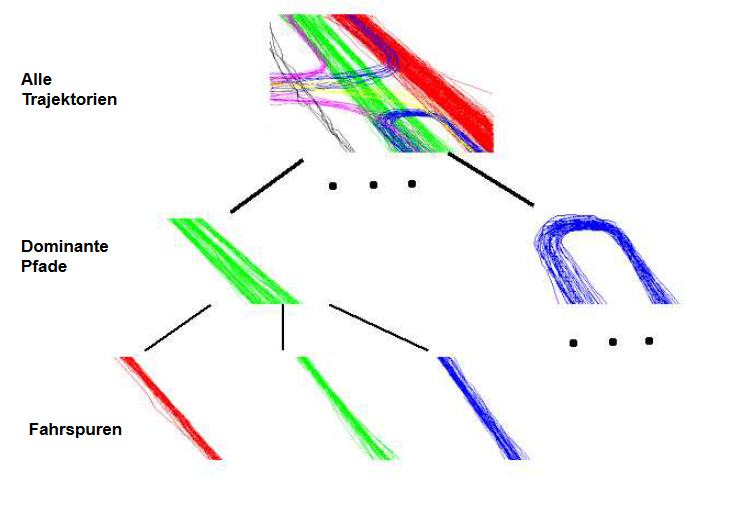
\includegraphics[width=0.5\linewidth]{../resources/img/RelatedWork/Fu_HierarchicalClustering}
    \caption[Zweistufiger Clustering-Vorgang von Hu et al.]{Zweistufiger Clustering-Vorgang von Hu et al. \cite[]{Hu2005}}
    \label{fig:relw_hu_two_step_cluster}
\end{figure}

Unter Verwendung des definierten Distanzmaßes werden die Trajektorien in einem zweistufigen Verfahren verarbeitet.
In den zwei Phasen werden, wie in Abbildung \ref{fig:relw_hu_two_step_cluster} dargestellt, zuerst dominante
Fahrpfade extrahiert, welche anschließend weiter in einzelne Fahrspuren untergliedert werden.
Als eigentliche Cluster-Algorithmen vergleichen die Autoren den \textit{Spectral-Clustering} Ansatz \cite[]{Ng2002}
mit einem \textit{Fuzzy-k-Means} Verfahren \cite[]{xie1991validity}.
Die Untersuchungen zeigen, dass der Spectral Clustering Ansatz nicht nur bessere Ergebnisse liefert, sonderen diese
über mehrere Durchläufe hinweg auch stabil sind, wohingegen die Resultate des Fuzzy-Ansatzes variieren.


% Junejo et al., 2004
\subsubsection*{Multi Feature Path Modeling for Video Surveillance}
Eine weitere Arbeit, welche das Ziel hat, anormale Bewegungsmuster auf Basis von Trajektorien zu entdecken,
stammt von \cite[]{Junejo2004}. In diesem Fall geht es den Autoren allerdings nicht um das Finden von Fahrzeug-Fahrspuren,
sondern um die Extraktion von Bewegungspfaden von Fußgängern.
Die Bewegungsbahnen der Passanten werden aus Aufnahmen stationärer Überwachungskameras gewonnen und
über zwei-dimensionale Punktreihen repräsentiert.
Als Ähnlichkeitsmaß für die Trajektorien verwenden die Autoren die Hausdorff Distanz. Die üblicherweise
negativen Eigenschaften dieses
Vergleichkriteriums (siehe Abschnitt \ref{sec:hausdorff_distance}), konkret die Missachtung der
Trajektorie-Orientierung, sind bei diesem Anwendungsfall kein Nachteil sondern ein Vorteil.
Da Fußgänger auf einem Pfad oder Weg in entgegengesetzte Richtungen gehen können, muss die Orientierung
ihrer Trajektorien ignoriert werden.
Auf Basis der Hausdorff Distanz erstellen Junejo et al. einen Graphen, in welchem die Knoten Trajektorien
und die gewichteten Kanten den Distanzen zwischen Trajektorien entsprechen.
Sie zerlegen diesen Graphen mit Hilfe des Graph-Cut Algorithmus und erhalten so die Cluster für die
extrahierten Fußgänger-Trajektorien.  


% Atev et al., 2010
%   Hier wiederum Erkennung von Fahrzeugtrajektorie-Clustern
%   Vorstellung eines neuen DM's (mod. Hausdorff) (--> Berücksichtigung Orientierung)
%   Vergleich von verschiedenen DM's und Cluster Algos (mod HD, LCSS(siehe Grundlagen), DTW)
%   Spectral-Clustering mit eig. mod. HD liefert nach Atev. beste Ergebnisse (ebenso Erweiterung zur Bestimmung von k)

% Chen et al., 2011
%   Clustering von Hurrikan Daten
%   Hier Orientierung ebenfalls relevant aber trotzdem Verwendung einfacher HD
%   Nicht relevant: Position der Trajektorien in Datensatz
%   Daher: Darstellung Trajektorien als Flow-Vektoren (Normiert!)

% Vlachos et al., 2002
%   Nicht metrisches Distanzmaß (Verschiebungen möglich) (LCSS basiert)
%   Für Erkennung von Zeichensprach Symbolen
%   Eig. sehr aufwendig. Beschreibung eines performanten Algorithmus
%   Kompliziert im Vergleich zu Chen et al.

% Melo et al., 2014
%   Weiterer etwas anderer Ansatz
%   Extraktion von Fahrzeugen und deren Position als Graph
%   Beschreibung von Trajektorien als Polynome niedrigen Grades (Meth. kl. Quadrate) (übl. 3te Grad)
%   Verwendung von rough-k-means Clustering um bereits Ausreißer (Spurwechsel) ausfiltern zu können
%   Einfache HD Distanz
%   Initiale Spur-Mitte über Aktivitäts Map bestimmt --> Vergleich der Spuren hierzu



\section{Erkennung von Fahrspuren}
\label{sec:rw_lane_detection}
% Hier Arbeiten vorstellen, welche (prim. auf Basis von Traj.Clustern) versuchen Fahrspuren / Fahrbahnen
% zu erkennen
% Auch übliche Ansätze vorstellen, welche nicht mit Traj. arbeiten (erwähnen häufig optisch / aus Fahrzeugen)

% Zuerst Ansätze, welche auf anderen (visuellen) Methoden basieren

% Melo et al.
%   repräsentiert Fahrspuren nur über Spurmittelpunkte (Clustering-Ergebnis)
%   Bestimmt Zugehörigkeit über Nähe zu Mittellinie 

% Chen et al.
%   Spur ebenfalls "nur" über Fahrbahnmittelpunkt repräsentiert.
%   Ermittelt über "polynom curve fitting" auf Clusterpunkte

% Fu et al. & Junejo et al.
%   Clustering und dann Bestimmung Envelopes basierend auf Varianz der Trajektorien in Cluster

% Hsieh et al., 2006
% Automatic Traffic Surveillance System for Vehicle Tracking and Classification

\section{Klassifizierung von Fahrspuren}
\label{sec:rw_lane_classification}

\section{Defizite vorhandener Lösungen und benötigte Neuerungen}
\label{sec:rw_deficites}

% Eigentlich nichts zur Spurerkennung auf bspw. Kreuzungen etc.
%   Wenn Spur dann immer nur Spur für gesamtes Cluster (kein Partitioning)

% Meiste Aufnahmen sind Frontal-Aufnahmen auf Straße --> keine Verzerrungen